\documentclass[12pt,oneside,final]{ucdthesis}

% need this for the \foreach command
\usepackage{tikz}
\dsp
% spacing in figures and tables and their captions can be
% changed here (\ssp for single-space, empty for same as surrounding
% text); for this to work, the command \figsp has to be included
% in every figure and table right after the \begin{figure}
% \def\figsp{\ssp}
%\def\figsp{}


% useful for drafts
% line numbers:
% http://www.ctan.org/tex-archive/help/Catalogue/entries/lineno.html
%
% \usepackage{lineno}

% customized headers
%
% http://www.ctan.org/tex-archive/help/Catalogue/entries/fancyhdr.html
% \usepackage{fancyhdr}

% a better verbatim environment: c/o Pete Dirac
% use like this:
%   \begin{Verbatim}[fontsize=8]
%       foobar
%    \end{Verbatim}
% \usepackage{fancyvrb}


% more flexible math support
\usepackage{amsmath}

% allow some pages to be landscape
\usepackage{lscape}

% more flexible definition of table environments
\usepackage{ctable}

%need this for \includegraphics{}
\usepackage{graphicx}
\graphicspath{{images/}}

%enable the listings package specifically for including programming code
\usepackage{listings}

%Special hack to make code listings not break pages, fyi they must be short then
\usepackage{float}
\floatstyle{plain} % optionally change the style of the new float
\newfloat{Code}{H}{myc}

%test alternative to listings package minted which requires the python pygments package
%minted was installed to latex by hand
%\usepackage{minted}

 % PDF links --- > breaks with some bibliography entries
% \usepackage{hyperref}

% nice looking, parenthetical references
%\usepackage[sorting=nyt,natbib=true,citestyle=authoryear,bibstyle=authoryear,maxnames=3,refsection
%=chapter,backend=bibtex]{biblatex}
%\usepackage{chapterbib} % incompatible with biblatex
%\bibliography{example}
%\defbibheading{bibliography}{%
%	\section{References}
%	}
	
% bibliography can be single-spaced for UC thesis format
%\appto{\bibsetup}{\ssp}
	

%make the index
% \usepackage{makeidx}
% \makeindex

% custom colors
\usepackage{color}
% make a color for comments
\definecolor{MyDarkBlue}{rgb}{0,0.08,0.45}

% customized captions with bold label and small, italic text
% table captions are located above tables
% http://www.kronto.org/thesis/tips/custom-captions.html
% http://www.ctan.org/tex-archive/macros/latex/contrib/caption/
% does this have any effect?
%\usepackage{caption}
% \renewcommand{\captionfont}{\small\itshape}
%
\usepackage[hypcap,font=singlespacing]{caption}
\usepackage{subcaption}
% modern method for setting up captions\
\captionsetup{margin=10pt,font=small,labelfont=bf}
%
% fix so that table captions have correct spacing
\captionsetup[table]{position=top}



% %
% %  fit more material on the page:
% %
%
% reset some float-controlling parameters
\renewcommand{\floatpagefraction}{0.8}	% require fuller float pages

% N.B.: floatpagefraction MUST be less than topfraction !!
\renewcommand{\topfraction}{0.9}	% max fraction of floats at top
\renewcommand{\bottomfraction}{0.8}	% max fraction of floats at bottom


% PDF formatting options, indexing, hyperlinking, with control over link style
%Set PDF Metadata
\usepackage[pdftex,
            pdfauthor={Author Name},
            pdftitle={Title Here},
            pdfsubject={Subject},
            pdfkeywords={Comma, List, Keywords},
            %pdfproducer={Latex with hyperref, or other system},
            %pdfcreator={pdflatex, or other tool}
            ]{hyperref}
\hypersetup{
	%driver=pdftex,
	colorlinks=true,
	urlcolor=blue,
	linkcolor=blue,          % color of internal links
    citecolor=blue,        % color of links to bibliography
    filecolor=magenta
}

%Use an additional package to make bookmarks point to the top to tables, figures and listings
\usepackage[all]{hypcap}

%Alex's customizations
\usepackage{indentfirst} %Indents first paragraph of chapter
\usepackage{datatool} %Allows import of csv and other data-tables
\usepackage{varwidth}
\usepackage{color}
\usepackage{rotating}
%\AtEveryBibitem{\clearfield{month}} %Cleaner references without month being printed

\usepackage[letterpaper, margin=1in]{geometry}
\setlength{\voffset}{0in}

% Macros:
\newcommand{\ASFJIRAURL}{\url{issues.apache.org/jira/}}
\newcommand{\timeperiod}{\textbf{T}}
\newcommand{\pd}[1]{{\scriptsize \todo{Prem:  {\color{blue} #1}}}}
\newcommand{\bm}[1]{{\scriptsize \todo{Ben:  {\color{magenta} #1}}}}

\usepackage{csvsimple}
\usepackage[turnon]{notes}
%%% Document Portion:
\begin{document}


%
%% Title, Front Matter, and Abstract:
% Declarations for Front Matter

% MS Thesis = 0, Phd Dissertation = 1
\isdissertation{0}

% electronic submission? Paper only = 0, Electronic = 1
\iselectronic{1}

\title{Organizational Social Networks in Apache Software Foundation Projects}
\author{Benjamin David Mishkanian}

% Choices are September, December, March, June
\degreemonth{September}
\degreeyear{2016}
%More examples DOCTOR OF PHILOSOPHY
\degree{Master of Science}

\chair{Premkumar Devanbu}
\othermembers{Vladimir Filkov,Cindy Rubio Gonz\'alez} %comma separated list of committee not including chair
\numberofmembers{3} % size of committee

\prevdegrees{B.S (University of California at Davis) 2014}

%Your Graduate Group
\field{Computer Science}
\campus{Davis}


% add the abstract here

% Their are two abstracts. One that is published externally from your
% dissertation, and one that is internal. Of course, the text of the
% abstract will be the same. So, we define a macro to hold the body of our
% abstract.
% at 345 words - With electronic filing there is no longer a word limit

\newcommand{\myabstract}{
put the abstract here
}


%Not required for electronic submission, you will need to print your other abstract page 2x and hand them in.
% Here is the first, external, abstract.
%\begin{abstract}
%	\myabstract
%	\abstractsignature
%\end{abstract}

\begin{frontmatter}
\maketitle

% A copyright page is optional. If you have one, it must immediately
% follow the title page. For more information about the copyright page
% see the UCD's Office of Graduate Studies web site.
% \copyrightpage

% dedication (optional), remove comment markers to use 
%\begin{dedication}
%\null\vfil
%{\large
%\begin{center}
%xxxx
%\end{center}}
%\vfil\null
%\end{dedication}



\tableofcontents
\listoffigures
\listoftables

% Here is the second, internal, abstract.
% Update: Melissa Danforth 2006
% Inline abstract is now part of front matter according to coordinator
    \newpage
    \begin{inlineabstract}
		%Only enable small if you're trying to make it fit.		
		%\begin{small}
		\myabstract
		%\end{small}
		
    \end{inlineabstract}

%Acknowledgments (optional)
\begin{acknowledgments}
xxxxxxx
\end{acknowledgments}

%Preface (optional)
\chapter*{Preface}
\addcontentsline{toc}{chapter}{Preface}
\input{preface}


\end{frontmatter}


%
% the chapters
%

% set page style:
% make the chapter and section smaller, chapter and section numbers are removed
% fancyplain will keep the page numbers at the bottom of all pages
%\pagestyle{fancyplain} %Note the \fancyplain command !!!
%\renewcommand{\chaptermark}[1]{\markboth{\small{#1}}{}}
%\renewcommand{\sectionmark}[1]{\markright{\small{#1}}{}}


% TODO: this is only for draft copies !!
% start line number printing
%
% \linenumbers



% chapter 1
\chapter{Introduction}
In recent years, there have been a variety of research papers analyzing the different facets of open source software (OSS). OSS research is of interest because if OSS has the potential to challenge the economics and methods of commercial development, as some have claimed, it is important to understand and evaluate it\cite{mockus2002two}. The success of several prominent open source projects have shown that the OSS development model can be highly productive. For example, Godfrey and Tu \cite{godfrey2000evolution} found that the Linux kernel project experienced superlinear growth over its six-year lifespan, in spite of prior research asserting that growth of software systems in general tends to slow down as they become larger. Further studies have been performed to identify specific benefits associated with open source projects. Paulson, et al. \cite{paulson2004empirical}, for instance, found empirical support for the hypothesis that "open source projects generally have fewer defects than closed source projects, as defects are found and fixed rapidly." The openness and decentralization of OSS projects can allow these projects to attain more developer attention than otherwise possible.

Although OSS projects are freely accessible to the developer community, it does not mean they are mutually exclusive with the interests of commercial organizations. In fact, a growing body of research has shown that the opposite is true. In a survey of developers of Java projects hosted on SourceForge, Capra et al. discovered that 31\% of the projects had a firm that was contributing in some way, with an average of two firms contributing per project\cite{capra2009survey}.

The time period \timeperiod{} under observation began at January 1, 2016 and ended at June 1, 2016. This period was chosen for two reasons:
\begin{itemize}
	\item A six-month period reduced the possibility of contributors having changed employers during the period, which would have introduced problems in cleanly associating their contributions with individual organizations.
	\item Since the LinkedIn employer data was collected in June 2016, having the period end at that time preserved the timeliness (and thus relevance) of that data.
\end{itemize}
 %This looks for chapter1.tex

% chapter 2
\chapter{Data Collection}

\section{Initial Research Question and Data Collection}
The original research question for this project was to identify differences in commit behavior between paid and volunteer contributors of open source projects. In order to classify contributors as paid or volunteer, a script was written which collects data from various public online profiles of ASF contributors active in 2015 and computes several heuristics which can then be used as features of a classifier. However, two issues made it difficult to identify the differences between the two classes:
\begin{enumerate}
	\item \label{manypaid} For a given ASF project and time period, the proportion of active contributors who are paid to work on the project can be very high, sometimes nearing 100%.
	\item \label{novolunteers} A profile can contain certain markers that are highly correlated with paid contributors, but there are no known markers that are highly correlated with volunteer contributors.
\end{enumerate}
Issue \#\ref{manypaid} was a surprising finding in its own right—we expected there to be a somewhat even mix of paid and volunteer contributors, but while doing a manual classification of a couple projects, we found these projects to be almost exclusively developed by employees of a few companies during the time period under observation. With such skewed samples, it became difficult to write a classifier sensitive enough to be useful.
Issue \#\ref{novolunteers} was an unforeseen limitation of using profile information to identify social group affiliation. Ultimately, there was no reliable way to differentiate between a volunteer and a paid contributor when his/her data does not reveal any obvious link between his/her contributions and his/her employer.
Although creating this classifier proved infeasible, we were able to re-purpose our data to do a social network analysis of ASF contributions instead. In particular, the following facets of the dataset were useful for this purpose:
\begin{itemize}
	\item The dataset associates data from multiple accounts/profiles to one contributor, improving the reliability of finding a given contributor’s employer.
	\item Since the contributor’s employer was one of the data points which the algorithm used, a fair amount of employer data was already available.
\end{itemize}

\section{Data Sources}
When researching open source software, there are a multitude of possible software repositories and organizations to base the experiment on. For example, some prior work studied SourceForge projects, while others studied GNOME. We chose to study Apache Software Foundation projects because they have a consistent organization structure with respect to how developers collaborate on Git, Github, and JIRA. This structure made it simpler to write a script that can reliably link user identities across these service.
To find the employer of a given Git committer, the script attempts to collect data from the Git account, and any associated JIRA and/or Github accounts. It also utilizes the Google Custom Search API to find links to LinkedIn profiles, which can then be inspected manually. Each set of values is stored in a separate entry in a PostgreSQL database, to maximize the amount of information available for finding a contributor’s employer.
The following information is mined from Git, Github, and JIRA accounts:
\begin{itemize}
	\item Username
	\item Email address
	\item Display name
\end{itemize}
The following additional information is mined from Git accounts:
\begin{itemize}
	\item Commit count per project
\end{itemize}
The following additional information is mined from Github accounts:
\begin{itemize}
	\item Location
	\item Company name
	\item List of organizations
\end{itemize}
Furthermore, to work around the rate limit of the Github API, we utilized a GHTorrent.org database dump as an offline cache of Github data.

\section{Data Collection Constraints}
Since a contributor’s employer name is information which can only be obtained if the contributor chooses to reveal it, there will typically be some individuals for which we have no employer name. A further constraint is that if this information cannot be mined automatically for most people, it becomes infeasible to fill missing values in the dataset through manual inspection. After performing some case studies, we found that this can be a significant problem for larger projects such as Apache Kafka, which have many individual committers. However, we found that the vast majority of commits to a project typically came from a small group of the committers, for which we could more easily find their employer. For this reason, we limited our data collection to only the prolific contributors of each project, defined as contributors in the minimum size set S such that the sum of the number of commits done by members of S is at least 80\% of the number of commits done to the project for the time period under observation. This also had the effect of improving the number of employer names mined automatically, because prolific contributors seem to be more likely to keep their Git, Github, and JIRA profile information up-to-date.
An additional constraint was that we only mined data for ASF projects that met the following constraints:
\begin{itemize}
	\item The project is listed in the GHTorrent.org database
	\item The project has a JIRA hosted at \ASFJIRAURL
	\item At least 20 commits were done to the project within the period under observation
\end{itemize}
These constraints resulted in the exclusion of projects which lacked sufficient data to analyze.
% TODO: do something about the overflowing table
\begin{table}
	\begin{tabular}{l|c}%
		\bfseries Organization & \bfseries Committers% specify table head
		\csvreader[head to column names]{companypeoplecount.csv}{}% use head of csv as column names
		{\\\hline\company & \personcount}% specify your coloumns here
	\end{tabular}
	\caption{Number of committers accounted for in each project}
\end{table}

\section{Data Collection Algorithm}
The script jiradb.py performs the majority of the data gathering. Its algorithm can be summarized as follows:
\begin{enumerate}
	\item Get JIRA account data for contributors to the JIRA of the projects
	\item Get Git account and commit data for committers to the projects
	\item Get Github account data for Git accounts
	\item Associate accounts belonging to a single person under a single contributor ID
\end{enumerate}
The following sections provide more details on these steps.

\subsection{JIRA Data}
The jira Python package was used to query the ASF JIRA at \ASFJIRAURL. JIRA can be queried programatically by using the JQL (JIRA Query Language). The following JQL query was used to download issues for project P that were either created or resolved in \timeperiod.
% TODO: replace format specifiers with actual values from mineProjects.sh
\begin{verbatim}
project = "P" AND created < "{1}" AND (created > "{2}" OR resolved < "{1}")
\end{verbatim}
\subsection{Git Data}
\subsection{Github Data}
\subsection{Identity Merging} %This looks for chapter2.tex

\chapter{Organizational Social Networks}
This chapter begins by presenting some background of social network methods in OSS research, and a description of how the organizational social networks were constructed. The social networks are then analyzed and discussed, using measures of centrality and centralization, along with some case studies of prominent clusters.
\pd{Begin each chapter (including this one) with a brief introductory summary sentence. e.g., In this chapter, we present some background on social network methods, and describe how we used them to analyze the interactions between companies and projects in the  Apache Software Foundation}\bm{Done.}

\section{Application of Social Networks to OSS Research}
In research projects concerning OSS, social networks are a useful tool to build understanding of the overall structure and flow of the distributed collaboration. Madey, Freeh, and Tynan\cite{madey2002open}, for instance, used social networks to perform an empirical study of collaboration on SourceForge projects, finding that the number of developers per project and the number of projects per developer both have power-law distributions. As another example, Bird, Gourley, Devanbu, Gertz, and Swaminathan\cite{bird2006mining} used social networks to analyze communication over the Apache HTTP server project's mailing lists, discovering a ``strong relationship between the number of messages sent, and the number of different people who respond to them,'' among several other findings.
\pd{Add one more example, e.g., the clustering work in Bird FSE 2007}. \bm{Done.}
 Similarly, by modeling organizational collaborations in ASF projects as a social network, we can answer questions about the high-level scope and structure of organizational involvement in ASF. 

For the present study, social networks were employed to find out the centralization level of organizational contributions to ASF, and to pinpoint the organizations which are most central to ASF project development. In addition to computing these values, the social networks were plotted using R, which provided a visual overview of the network structure. Afterwards, some of the most interesting phenomena observed in these network analyses were investigated in more detail, in order to better understand what caused them to appear, and what effects they had on the network.
\section{Building the Network}
Once the contributors' commit counts and employers were known, a social network of organizations was created based on the shared collaborations of their members. This was done in the following steps:
\begin{enumerate}
	\item The \textbf{companyprojectcommitcount} table was joined with itself on column \textbf{project} and the two commit counts of each row were summed into one, creating an edge list for organizations, with the summed commit count as the edge weight.
	\item The edge list was imported into R, and symmetric edges created by the join were removed.
	\item If two edges connected the same pair of vertices (caused by two organizations being connected through multiple projects), the edges were merged by summing their commit counts. 
	%\pd{Briefly explain why multiple edges may arise between a single pair of nodes} \bm{Done.}
	\item Networks were created using R packages \textbf{network} and \textbf{igraph}.
\end{enumerate}
Essentially, there was an undirected edge between organizations A and B when a member of A and a member of B contributed to the same project. The edge weight was the sum of the number of commits from A's members and the number of commits from B's members to all projects where they both contributed.

\section{Network Plots}
One challenge in plotting complex networks is that when there are many nodes and edges, it becomes difficult to discern the structure of a network by looking at the plot, especially if it was plotted using a simple algorithm. Since the organizational network had 90 vertices and 622 edges, a more sophisticated plotting approach was necessary. In their 2004 paper\cite{gonzalez2004community}, Gonz{\'a}lez-Barahona, L{\'o}pez, and Robles demonstrated that the Girvan-Newman (GN) algorithm, which can be used to generate a hierarchical graph layout, making it easier to visually identify graph structure. They applied this method to plotting a network of developers of the Apache HTTP Server, the founding project of the ASF, and asserted that the GN algorithm provides ``a step forward at least in the aspect of offering a way to visually identify an affiliation network,'' compared to the classical network analysis algorithms used by previous works. Since the GN algorithm was shown to be effective for highlighting the structure of the Apache developer network, it was applied for plotting the ASF organizational network.

An image of the plot is shown in figure \ref{fig:orgCommunities}. This plot was generated using the R package \verb|igraph|, which contains a function named \verb|edge.betweenness.community| that implements the GN algorithm to generate a ``communities'' object. Communities highlight graph structure by grouping vertices into different neighborhoods based on their edges. In the figure, each community is shaded with a different color, and vertices in the same community are colored the same, making it easier to see the relationships between clusters. Edge weights are not reflected in this graph, as the vertices could not be spread out far enough to allow increasing edge thickness without causing disruption. The number of contributing members in an organization is reflected in the vertex size.

In looking at the graph, it is immediately apparent that there are identifiable clusters of organizations that are in close collaboration, and there are a few ``linchpin'' organizations which connect these clusters. Although the center cluster is still a bit too cluttered, the easy identifiability of the communities and the vertices connecting them provides further evidence that hierarchical algorithms such as GN are well-suited for the task of exhibiting the structure of complex social networks. A closer analysis of the clusters is provided in section \ref{clustersection}.
\begin{figure}
	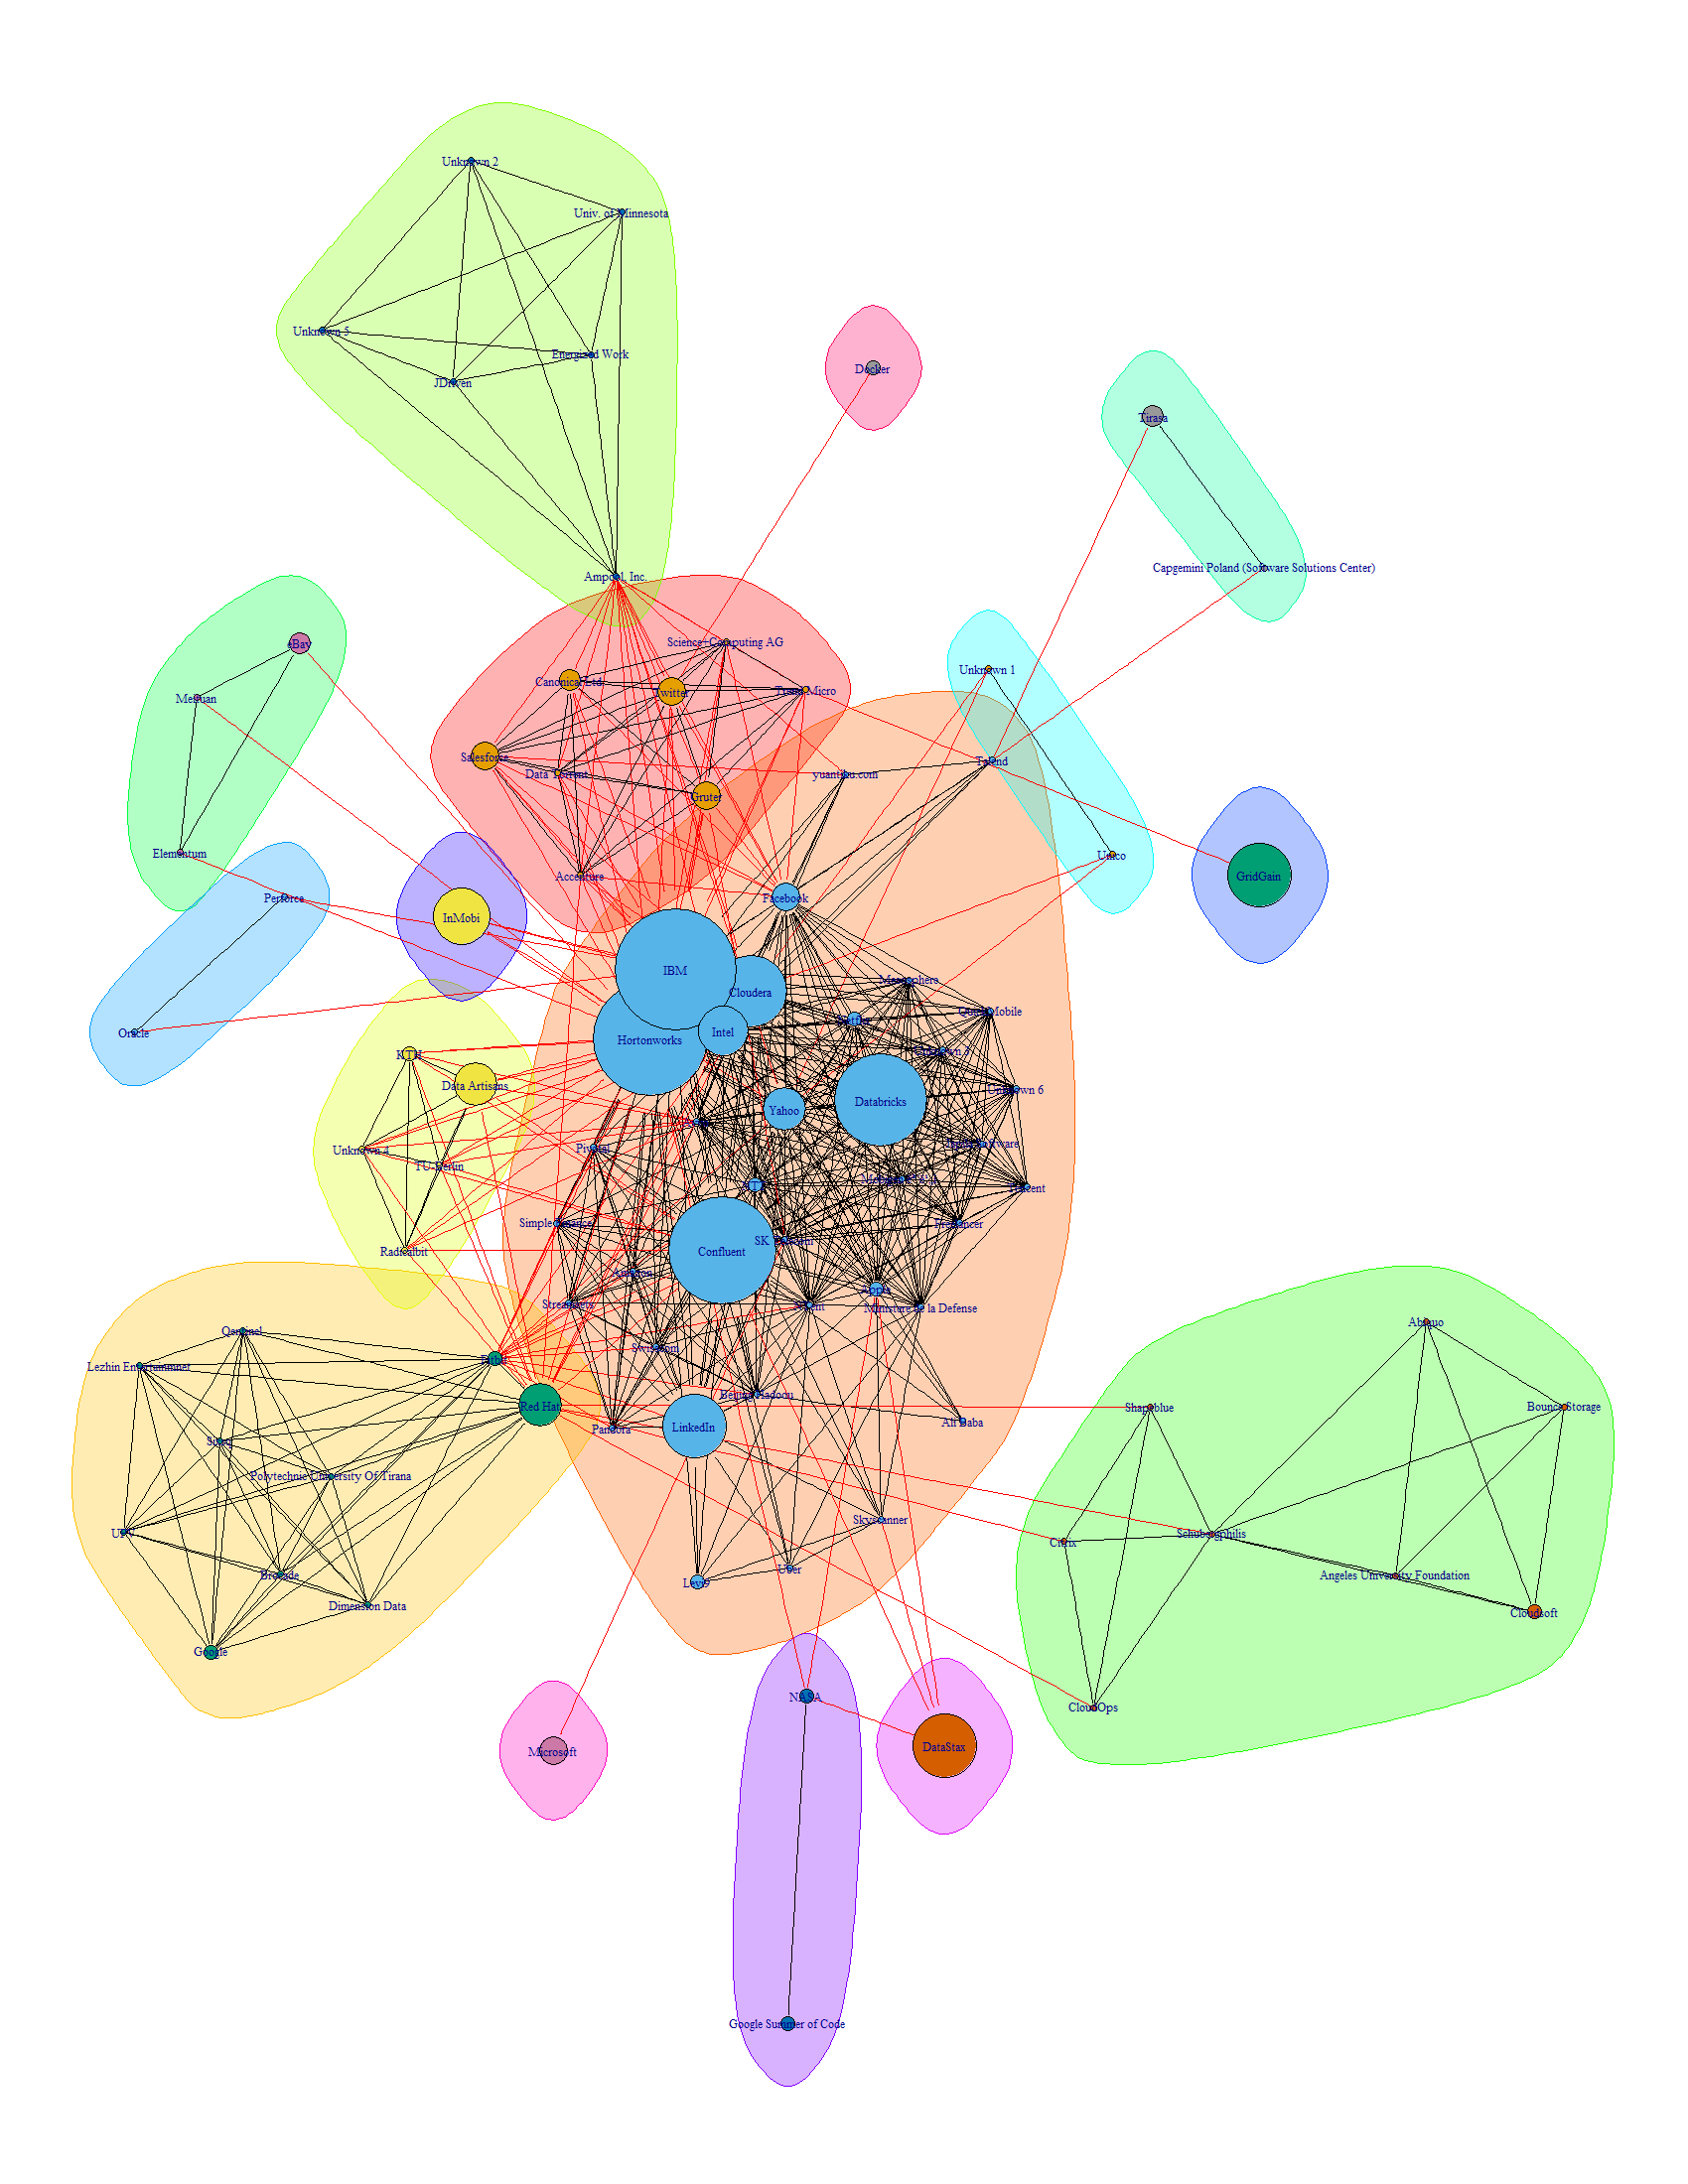
\includegraphics[width=\textwidth]{communities.png}
	\centering
	\caption{The organizational communities}
	\label{fig:orgCommunities}
\end{figure}

\section{Centrality and Centralization Measures}


Measuring the centrality of nodes in a network can be an effective way to learn about the network structure. As a review, the following discussion includes definitions of centrality and centralization, taken from \textit{Introduction to social network methods}\cite{hanneman}.

The centrality of a vertex is a measure of how close it is to the ``center of action'' in a network. There are multiple different ways to measure centrality, but the most common are degree centrality, closeness centrality, and betweenness centrality. Each of these was computed for all vertices in the organizational networks. The next three subsections provide more detail on these measures, followed by a discussion on the centralization of the network as a whole.

\subsection{Degree Centrality}
Degree centrality is measuring centrality using the degree (i.e. the number of incident edges) of a vertex. For directed graphs, degree can be measured using indegree, outdegree, or the sum of the two. Since the organizational network is an undirected graph, all edges incident to a vertex were counted in the degree. The following formula was used to calculate degree centrality of vertex v in graph G, where V(G) and E(G) are the vertices and edges of G, respectively \pd{explain what V(G) and E(G) is}\bmdone{Done.}: 
\begin{equation*}
C(v) = | {i\:in\:V(G) : (i,v)\:in\:E(G)} |+|{i\:in\:V(G) : (v,i)\:in\:E(G)}|
\end{equation*}
This is the ``Freeman'' degree---the sum of the indegree and outdegree of the vertex v. A table of the organizations with the highest degree centrality is shown in table \ref{tab:degree}.
%  \pd{Provide a fomula for degree centrality}. \bm{Done.}

\begin{table}
	\begin{tabular}{l|c}%
		\bfseries Organization & \bfseries Degree% specify table head
		\csvreader[head to column names]{degree.csv}{}% use head of csv as column names
		{\\\hline\organizationa & \scorea}% specify your coloumns here
	\end{tabular}
	\centering
	\caption{The 10 organizations with the highest degree centrality}\label{tab:degree}
\end{table}
\subsection{Closeness Centrality}
Closeness centrality is a measure of how ``close'' a vertex is to all others in the network. For the present study, the closeness of two vertices was computed using the following formula:
\begin{equation*}
	C(v) = (|V(G)|-1)/sum( d(v,i),\:i\:in\:V(G),\:i \neq v )
\end{equation*}
where d(i,j) is ``the geodesic distance between i and j (where defined)''\cite{butts}. A geodesic is the shortest path between two vertices. If there is no path between the vertices, the geodesic is undefined. 
%\pd{Explain geodesic, and when it might not be defined} \bm{Done.}

A table of the organizations with the highest closeness centrality is shown in table \ref{tab:closeness}. Unlike degree centrality, closeness centrality takes into account the distances to vertices that are more than one edge away. This means that vertices raking high in closeness centrality are central to the network as a whole, rather than simply central to their neighborhoods. For example, SK Telecom has low closeness, but high degree. Looking back at the visualization in figure \ref{fig:orgCommunities}, we can see this is because it is directly in the center of the large central cluster, which provides it many direct edges, but insulates it from all other clusters. In the other extreme, Fitbit has high closeness but relatively low degree, because although it has short paths to most clusters, it achieved this through a small number of links to other linchpin organizations. Still, eight out of the ten organizations are included in both lists, so already a pattern begins to emerge about which organizations are most central overall.

\begin{table}
	\begin{tabular}{l|c}%
		\bfseries Organization & \bfseries Closeness% specify table head
		\csvreader[head to column names]{closeness.csv}{}% use head of csv as column names
		{\\\hline\organizationb & \scoreb}% specify your coloumns here
	\end{tabular}
	\centering
	\caption{The 10 organizations with the highest closeness centrality}\label{tab:closeness}
\end{table}

\subsection{Betweenness Centrality}
%\pd{Need to provide a more formal definition of how it is calculated} \bm{Done.}
Betweenness centrality is a measure of how frequently a vertex appears in the list of shortest paths between all other vertices. Stated differently, it measures how likely it is that vertex V must be traversed when taking the shortest path between arbitrary vertices A and B. Betweenness places more emphasis on the importance of edges than closeness does; an edge that is on many shortest paths is likely to confer high between centrality scores on its incident vertices. The betweenness of a vertex was computed using the following formula:
\begin{equation*}
C(v) = sum( g_{ivj} / g_{ij},\:i,j: i \neq j,i \neq v,j \neq v )
\end{equation*}
where $g_{ijk}$ is ``the number of geodesics from i to k through j''\cite{butts}. 

A table of the organizations with the highest betweenness centrality is shown in table \ref{tab:betweenness}. One change that immediately stands out is that Red Hat is ranked second, whereas in the other two rankings it was not even in the top ten. This can be explained by taking another look at figure \ref{fig:orgCommunities}. At first glance, Red Hat seems to have similar positioning to Fibit, in that it has a medium number of edges to some other important actors. However, the difference is that Fitbit's direct connections are all in the 3 clusters nearest to it, whereas Red Hat has far-reaching connections to several clusters on the other side of the graph. This means that the shortest paths between nodes at the periphery of the graph are much more likely to require use of Red Hat's edges, because it is an efficient bridge between clusters, compared to Fitbit's edges.

% This does not escape special characters--be careful with ``Ampool, Inc.''
\begin{table}
	\begin{tabular}{l|c}%
		\bfseries Organization & \bfseries Betweenness% specify table head
		\csvreader[head to column names]{betweenness.csv}{}% use head of csv as column names
		{\\\hline\organizationc & \scorec}% specify your coloumns here
	\end{tabular}
	\centering
	\caption{The 10 organizations with the highest betweenness centrality}\label{tab:betweenness}
\end{table}

\subsection{Centralization}
Centralization measures the amount of variability in the centrality of the vertices of a network. It is a statistic of the network, rather than the individual nodes. A network with high centralization is one in which there is an unequal distribution of centrality in different parts of the network.  Centrality was computed for the organizational network using the following formula, developed by Freeman\cite{freeman1978centrality}:
\begin{equation*}
C^*(G) = sum( |max(C(v))-C(i)|,\:i\:in\:V(G) )
\end{equation*}
This formula requires some function C to measure centrality of vertices, and since there were three available methods to measure centrality, there are three different computed values for the network centralization. Table \ref{tab:centralization} displays the centralization value for each centrality measure. These values can be interpreted as percentages of centralization, with 1.00 indicating a completely centralized graph where only one vertex is central.

The difference between the centralization values computed when using closeness versus betweenness for measuring centrality is striking. This discrepancy was likely caused by the fact that most of the vertices had a betweenness value of zero, making most of the summands in the centralization formula zero as well. Indeed, from the perspective of betweenness centrality, the network truly does appear somewhat decentralized, because the majority of the nodes are not on any shortest paths, and thus they are equally low in betweenness centrality. However, the nodes that are high in betweenness centrality have extremely high scores in it, keeping the network centralization above 25\%. Due to the skewness of the betweenness centrality distribution, this is likely somewhat of an underestimate. After all, a visual inspection of the graph makes it readily apparent that the central cluster would cause very high centralization, if nodes such as Red Hat and Fitbit did not provide alternative bridges between clusters. The average of the three centralization value is 43\%, so we can roughly estimate that the centralization level of the organizational network is somewhere between 25\% and 50\%, which is moderately centralized. The effects of this centralization are discussed in the next chapter.

\begin{table}
	\begin{tabular}{l|c}
		\bfseries Centrality Type & \bfseries Centralization \\
		\hline
		Degree & 0.4905946 \\
		\hline
		Closeness & 0.5550736 \\
		\hline
		Betweenness & 0.2619162
	\end{tabular}
	\centering
	\caption{The network centralization value for each centrality measure}\label{tab:centralization}
\end{table}

\section{Cluster Analysis}\label{clustersection}
The GN algorithm identified sixteen communities, or clusters, in the organizational network. Since there were forty projects, the relatively low number of clusters suggests that the grouping algorithm is more sophisticated than simply grouping organizations with their main projects. (The average number of projects per organization was 1.95, with a median of 1, so a simple project-based grouping algorithm would likely create too many clusters to be useful\footnote{See table \ref{tab:orgprojects} in appendix \ref{ch:orgdata} for the full data of project count per organization.}.) At the same time, it created enough clusters to prevent the graph from devolving into a few large blobs. (For comparison, the greedy algorithm \textbf{fastgreedy.community} only created five clusters.)
 \pd{The previous sentence needs more details and justification. Add a few sentences explaining why you find that GN is doing something sophisticated}\bm{Hopefully this explains it better. I also weakened the claim a bit.}
  Still, project collaborations are what the network is based on, so as a first attempt at understanding these clusters, table \ref{tab:clusterprojects} relates clusters with the projects where most of the cluster's organizations contribute.\pd{Don't end sentences a proposition with :-)}\bm{I see what you did there :) Fixed.}

\begin{table}
	\begin{tabular}{l|c}
		\bfseries Cluster & \bfseries Associated Projects \\
		\hline
		Salesforce, Gruter, etc. & bigtop \\
		\hline
		Docker & aurora \\
		\hline
		DataStax & cassandra \\
		\hline
		Shapeblue, Citrix, etc. & cloudstack \\
		\hline
		NASA, Google Summer of Code & climate \\
		\hline
		Unico, Unknown 1 & curator \\
		\hline
		Hortonworks, Confluent, etc. & spark, storm, kafka, oozie, bigtop, flink, hbase, samza \\
		\hline
		Data Artisans, KTH, etc. & flink \\
		\hline
		Red Hat, Fitbit, etc. & libcloud \\
		\hline
		Microsoft & reef \\
		\hline
		GridGain & ignite \\
		\hline
		InMobi & lens \\
		\hline
		Oracle, Perforce & derby \\
		\hline
		eBay, Elementum, Meituan & kylin \\
		\hline
		Tirasa, Capgemini Poland & cxf \\
		\hline
		JDriven, Ampool, etc. & groovy
	\end{tabular}
	\caption{The projects associated with each cluster}\label{tab:clusterprojects}
\end{table}

Evidently, most clusters have one main project that they are closely associated with, with the only exception being the center cluster, which is associated with several projects. The relatively large number of projects controlled by the central cluster goes a long way in explaining why the cluster is so large and complex. Digging deeper into the original dataset, it was revealed that the major actors in this cluster, such as Hortonworks, contributed to most or all of the projects in this cluster, implying that the projects are closely related. The fact that these organizations are actively contributing to so many projects is likely related to the fact that many of these organizations are some of the largest in the network in terms of member count. One interesting question for future work is to determine what causal relationship (if any) exists between these two observations.

\chapter{Results}
This chapter reviews the results of the experiment, also providing interpretations which could be used as hypotheses for further studies. The answers to the research questions posed in chapter 1 are also discussed here.

\section{Centralization}
One of the primary research questions of this study was whether commercial development of OSS is highly centralized. Since ASF is only one community of the broader OSS development community, in order to apply the results of the present experiment to OSS in general, an assumption must be made that ASF has similar organizational dynamics to most other OSS communities. As this has not yet been proven, the following results are presented as pertaining to ASF in particular.

The centralization of the organizational network was estimated to be between 0.25 and 0.50, based on three different measures of centrality. In comparison, Crowston and Howison\cite{Crowston2006} studied interaction networks of developers in bug tracking systems on SourceForge, ASF, and Savannah, finding a wide range of centralizations within different projects, ranging from near 0 to near 1, with a mean of 0.54. In light of their findings that extreme values of centralization and decentralization are commonplace in OSS social networks, the centralization values of the organizational network can be considered moderate in this context.

One way to interpret high centralization in a network is to say the ``balance of power'' in the network is not evenly distributed. There are potential advantages to being a central node in a centralized network. For example, if the organizational network's edges are considered to represent the flow of knowledge between organizations, then all knowledge flowing between JDriven and the other clusters flows through Ampool first. This gives Ampool power over JDriven, because it has access to knowledge external to their cluster, and it may or may not share that knowledge. Stated in more concrete terms, Ampool has acquired knowledge by contributing to project bigtop, and it also contributes to project groovy, along with JDriven; however, Ampool is the only contributor to groovy that also contributes to other projects, so Ampool has the potential to be a valuable source of knowledge to the groovy contributors, due to its broader knowledge of other projects. If Ampool shares new information about tools, design patterns, or methodologies, for instance, it can aid groovy development. Although such information is not wholly inaccessible to the other groovy contributors otherwise, Ampool's experience with other projects can facilitate the knowledge flow. Further experiments are necessary to evaluate the extent to which such knowledge flow takes place, and what other variable affect it. Even so, it can be assumed that centrality in the network is advantageous to organizations because it at least provides them the \textit{potential} of increased access to information, regardless of whether or not it is realized.

Since the organizational network is moderately centralized, it implies there exist certain disadvantages for organizations that exist on the periphery of the network. These organizations are typically on the outskirts because they contribute to only one or two projects, where there are few other organizations contributing. Such isolation from other organizations can make the aforementioned knowledge sharing difficult. In turn, this can reduce the visibility of the projects, an instance of the ``rich get richer'' effect that is often associated with centralized networks. This is not to say that it is always better to contribute to the ``popular'' projects; rather, it is a suggestion that there is value in contributing to multiple projects, even if the additional projects are only indirectly related to the organization's operations. The fact that all clusters in the network are connected shows that some organizations have found reasons to contribute to projects that the other members of their cluster ignored. In doing so, they became linchpins. Of course, some organizations may not have the resources to contribute to multiple projects, but for those that do, the potential benefits of doing so in this centralized network should be taken into consideration.

\section{Central Organizations}
Another goal of this study was to find out which organizations are central to OSS development. Three different methods of calculating centrality were applied to the nodes in the organizational network, and the full results are shown in the tables in appendix \ref{ch:centralities}. By each measure, Hortonworks is the most central organization, but there was some variation for the rest of the results.

As a case study, Hortonworks' contribution patterns were examined in more detail to find out why it is so central. One of Hortonworks' core products, Hortonworks Data Platform, is built on top of 22 ASF projects\cite{hdp}, which explains why it has so many connections in the network. In addition, these projects are closely related in terms of domain and usage. Table \ref{tab:centralclusterprojects} summarizes the primary purpose of each of the projects associated with the central cluster, of which Hortonworks is a member. Clearly, they are all ``Hadoop related'' projects\cite{hadoopecosystem}, supporting the Hadoop ecosystem of large-scale distributed data processing.

\begin{table}
	\begin{tabular}{l|l}
		\bfseries Project & \bfseries Purpose \\
		\hline
		spark & large-scale data processing engine\cite{spark} \\
		storm & distributed realtime data processing\cite{storm} \\
		kafka & scalable distributed messaging system\cite{kafka} \\
		oozie & ``workflow scheduler system to manage Apache Hadoop jobs''\cite{oozie} \\
		bigtop & ``packaging, testing, and configuration\textellipsis{}of big data components''\cite{bigtop} \\
		flink & ``distributed stream and batch data processing''\cite{flink} \\
		hbase & ``distributed, scalable, big data store''\cite{hbase} \\
		samza & ``distributed stream processing framework''\cite{samza}
	\end{tabular}
	\centering
	\caption{The projects associated with the central cluster}\label{tab:centralclusterprojects}
\end{table}

Hortonworks was the only organization that contributed to all of these projects during \timeperiod, but several of the organizations with the highest centralities contributed to many of them. For example, Confluent and IBM each contributed to five of the eight projects, and Cloudera and Yahoo each contributed to four. Additionally, most of the organizations that provide the largest numbers of active contributors are primarily contributing to these projects. Evidently, a significant chunk of the total contemporary development effort in ASF is focused on the Hadoop ecosystem, both in terms of the number of organizations contributing, and also the number of contributors per organization. Due to the overall centrality of the Hadoop related organizational cluster, the type of projects an organization contributes to is currently a big factor in determining its centrality. However, since this experiment observed only one section of time, it is unknown whether this type of domain-dominated centrality was prevalent in the past, or will continue to be in the future.

As stated previously, the existence of ``bridge'' organizations such as Red Hat helps to lower the network centralization, because they provide short paths between clusters. The question is, why do these organizations contribute to projects not associated with their own clusters, while most of the others generally stick to projects associated with their clusters? Digging deeper into Red Hat's contributions helped to shed some light on the answer: Red Hat sells private cloud infrastructure-as-a-service\cite{redhat}, so unsurprisingly it contributed to cloud related ASF projects such as cloudstack and libcloud. Cloud computing is a different domain from the distributed computing promoted by the Hadoop ecosystem, but it shares some of the scalability challenges. This may be why Red Hat also contributed to flink and mahout, two projects which support scalable computing. In doing so, it became a bridge between the cloud related cluster and the Hadoop related one. Further research is necessary to evaluate whether projects with broader domains truly are catalysts for increasing knowledge flow between organizational clusters.

\chapter{Conclusion}
This thesis presented several findings about how organizations contribute to Apache Software Foundation projects. A social network was used to model the collaborations between organizations, allowing both visual and mathematical analysis of the structure of the ASF from an organizational perspective. The network was found to be moderately centralized, with a central cluster of Hadoop related collaboration being one of the main features of the network. It was also shown that a few organizations achieved high centrality not by existing in the central cluster, but by connecting multiple disparate clusters.

\pd{Some discussion of why this matters. E.g., useful to know what the clusters of related businesses are; which businesses play central roles overall, and in each cluster; which businesses are playing "gateway" or brokering roles. This important could be useful for both people considering use or actually using this software (why?) for investors (why) for job-seekers (why?) and for employers (why?)}. 

\pd{Actually add comments relating to the importance of your conclusions, as related above,  at the appropriate places in chapter 4}. 

These findings have implications for how individuals and organizations that are interested in the ASF. First of all, it was shown that organizations play a very significant role in the ASF, with some projects having substantially all of their commits during the observed period authored by employees of a single organization. Second, the centralization of the organizational network was discovered to be moderate, meaning that there may be a significant disparity in knowledge flow or other benefits experienced by two organizations contributing in different areas of the ASF. Third, it was revealed that the most central cluster of organizations is closely related to development of the Hadoop ecosystem, which provides insight into how much Hadoop has become central to the ASF as a whole; work on distributed computing in general comprised a large chunk of ASF development in 2016 thus far.

% TODO: Future work:
% - Take into account the time component (split into epochs, see changes over time).

% note that the 'plainnat' style does not allow URL's in the bibtex entry
%
% some ideas here:
% http://bib2web.djvuzone.org/bibtex.html
%

% reset the page style
%\pagestyle{plain}

\bibliographystyle{plain}
\bibliography{example}

% To enable this it will need to be added to toc so it's not in a chapter
%\printbibliography[heading=bibliography]

% the appendix:
% there are several sections, that don't really fit into the main chapters
%
\part*{\addcontentsline{toc}{part}{Appendices}Appendices}
\appendix

% reset page style to fancy
%\pagestyle{fancyplain}

 \chapter{Centrality Scores}
\DTLloaddb{degtab}{fulldegree.csv}
\begin{longtable}{l|c}
	\caption{Degree centrality of organizations}\label{tab:fulldegree}\\
	\bfseries Organization & \bfseries Degree
	
 \DTLforeach{degtab}{%
	  	\organization=organization,%
	  	\score=score%
 }{%
 \\\hline\organization & \score
	}
\end{longtable}

\DTLloaddb{bettab}{fullbetweenness.csv}
\begin{longtable}{l|c}
	\caption{Betweenness centrality of organizations}\label{tab:fullbetweenness}\\
	\bfseries Organization & \bfseries Betweenness
	
	\DTLforeach{bettab}{%
		\organization=organization,%
		\score=score%
	}{%
	\\\hline\organization & \score
}
\end{longtable}

\DTLloaddb{clotab}{fullcloseness.csv}
\begin{longtable}{l|c}
	\caption{Closeness centrality of organizations}\label{tab:fullcloseness}\\
	\bfseries Organization & \bfseries Closeness
	
	\DTLforeach{clotab}{%
		\organization=organization,%
		\score=score%
	}{%
	\\\hline\organization & \score
}
\end{longtable}


\end{document}
